\chapter{1T' $WSe_2$ state of the art}

\section{Introduction}
In contrast to other 2D materials like hBN or graphene, TMDCs exhibit structural polymorphism and as such open an additional avenue in 2D material engineering. The relation between different phases observed in TMDCs can be seen in Figure \ref{fig:1T'TMDCPhases}. On top of altering the electronic nature of the TMDC, semiconducting or metallic, there can also be observed a variety of superconducting states \cite{Saito2015}\cite{Lu2015}, quantum spin Hall insulators \cite{Qian2014}\cite{Choe2016}\cite{Liu2016a}\cite{Fei2017} or Weyl semimetals \cite{Sun2015}. Interestingly the various TMDC phases can coexist at specific temperatures and pressures \cite{Kappera2014}\cite{Keum2015}\cite{Cho2015}. Those different phases can exhibit small difference in energy per formula unit $MX_2$. As such a phase transition can be induced via e.g. a charge injection \cite{Duerloo2014}. Overall the various phases of the TMDCs and the transitions between are of great interest and remain unexplored in full detail.
The monolayers of TMDCs can be usually found in either 1H or 1T phase where the exact configuration depends on the thermodynamics \cite{Keum2015}\cite{Cho2015}. In order to identify which of those phases is more favourable the crystal field theory can be applied. The number of electrons in d orbitals of transition metals needs to be counted for a given TDMC material. For group 4 TMDCs (Ti, Zr and Hf) that number is 0 ($d^0$) while for group 10 (Ni, Pd and Pt) the number is 10 ($d^6$). It can be therefore shown that the number of electrons in d orbitals correlates with the phase transitions in TMDCs as seen in Figure \ref{fig:1T'EnergyDiagram}. The group 4 TMDCs ($d^0$) for instance are most stable in 1T phase. However the $d_{z^2}$ level of the 1H phase has the lowest energy and therefore the TMDCs of group 5 ($d_1$) and group 6 ($d_2$) fill that level first and therefore, they group 5 TMDCs are found most stable in  either 1T or 1H phase while the group 6 TMDCs are most favourable in 1H. After filling the $d_{z^2}$ level in group 6 TMDCs, the additional electron in group 7 TMDCs contribute to the 1T levels and results in a distorted octahedral coordination (1T') with clusterisation or Peierls distortions of the metal atoms. Furthermore the group 9 and 10 TMDCs are most stable in the regular octahedral coordination (1T).

\begin{figure}[!h]
	\begin{center}
		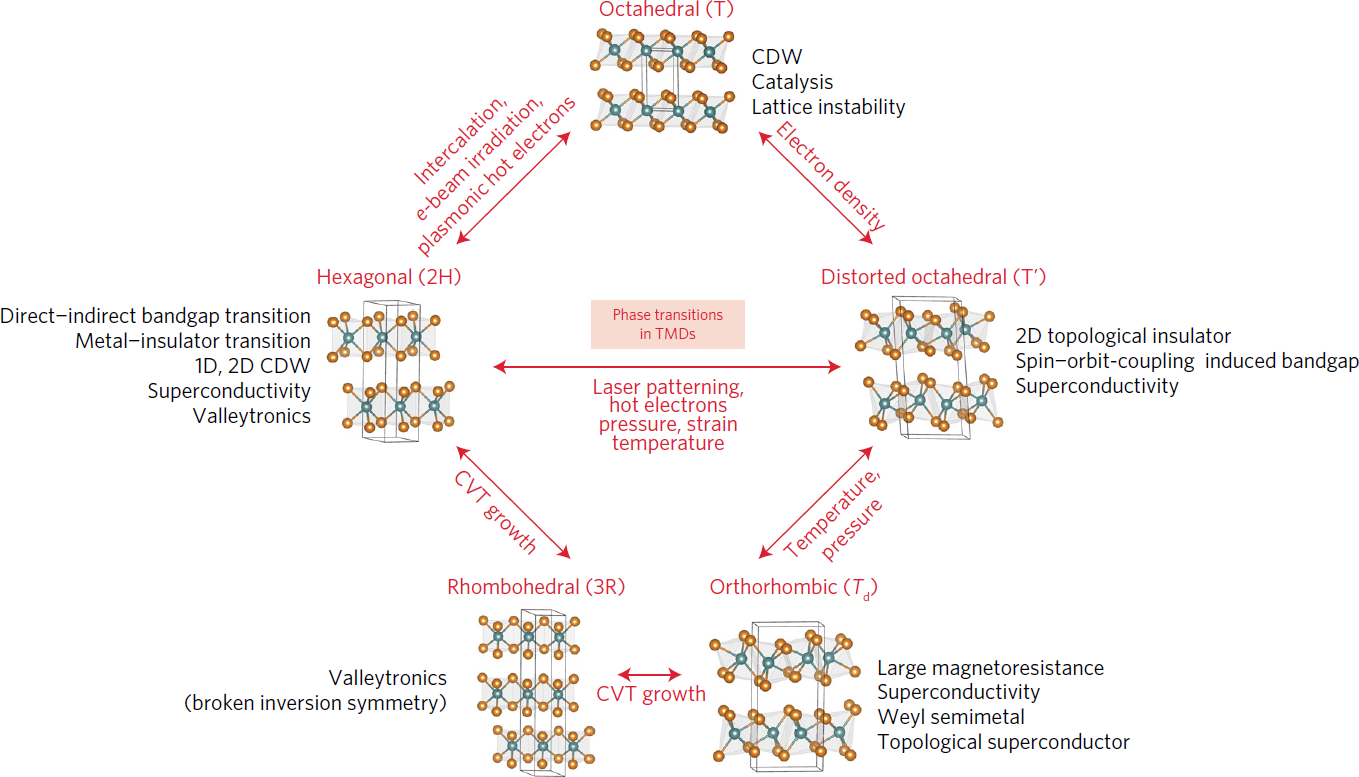
\includegraphics[scale=0.3]{1T'/TMDCPhases.png}
		\caption{Transition and correlation between phase and physics in TMDCs. Reproduced from \cite{Yang2017}}
		\label{fig:1T'TMDCPhases}
	\end{center}
\end{figure}

\begin{figure}[!h]
	\begin{center}
		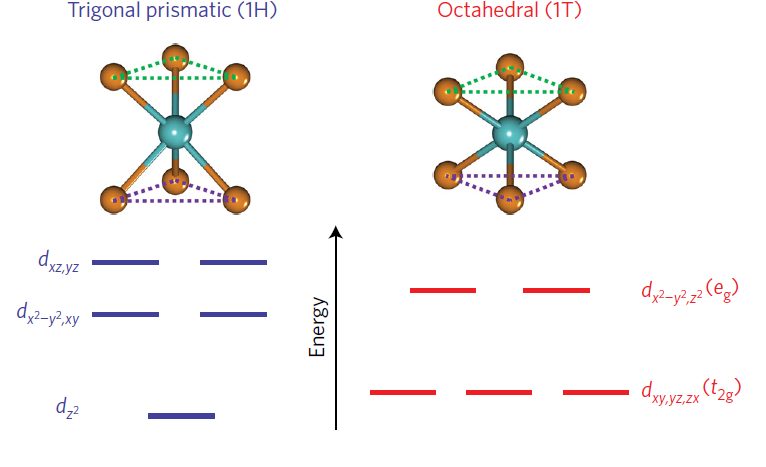
\includegraphics[scale=0.5]{1T'/EnergyDiagram.png}
		\caption{Schematic images of 1H and 1T lattice symmetries and energy levels of d-orbital electrons induced by the crystal field. Reproduced from \cite{Yang2017}.}
		\label{fig:1T'EnergyDiagram}
	\end{center}
\end{figure}

Recently the 1T' phase has received attention due to the predictions of potential Weyl semimetal or quantum spin Hall effects for group 6 TMDCs \cite{Qian2014}\cite{Sun2015}. Additionally the lattice distortion orientation can be affected by strain which allows for mechanical control of ferroelasticity and potential application as a shape memory material \cite{Li2016}. In order to achieve those effects in group 6 TMDCs a phase transition from 1H to 1T' generally has to be occur \cite{Chhowalla2013}. Such transition is usually performed via the lithium intercalation or chemical exfoliation. Following the lithiation the excess of the electrons is found in the d orbitals of the transition metals. As a result of that the electron density of those orbitals increases from $d_2$ to $d_{2+x}$. In order for a full transition from 1H to 1T to occur the excess of the electrons must be in range of 0.2 to 0.4. However if the excess is smaller than that then the distortion of the lattice may help to accommodate the phase transition.

One of the most important characteristics of TMDCs that influences a myriad of different properties is the number of layers. Especially in case of optical and electronic properties of 2H TMDCs the number of layers strongly affects the size and the nature of the bandgap, transitioning from indirect in bulk to direct in monolayer. The number of layers is however also of crucial importance to quantum effects observed or predicted in TMDCs in that the bulk material exhibits the in-plane inversion symmetry while the monolayers break it \cite{Saito2015}\cite{Lu2015}. Such breaking of symmetry leads to strong spin-orbit coupling as well as effective Zeeman fields in TMDCS. Additionally and out of plane spin polarisation which depends on the valley, K or -K point, has been observed when a strong anisotropic magnetic field has been applied to quench the superconductivity in 2H-$MoS_2$. There has also been observed a superconducting state in monoclininc and 1T' $MoTe_2$, and where also the Weyl semimetal and topological insulator states are expected \cite{Qian2014}\cite{Sun2015}\cite{Qi2016}.

Due to the distortion in the 1T' phase of the group 6 TMDCs a band inversion near the Fermi level with p and d bands from chalcogenides and metal atoms respectively. These bands result in some interesting phenomena, the Weyl state and quantum spin Hall effect. Those effects can manifest themselves in distorted octahedral phase (1T') or ortorhombic ($T_d$) phase. It has been shown using DFT calculations that group 6 TMDC in the T' phase exhibit the band inversion resulting in the quantum spin Hall effect \cite{Qian2014}\cite{Choe2016}. The change in number of layers results not only in inversion symmetry breaking but also affects the bandgap magnitude and as such is crucial in achieving the dissipationless spin transfer by the QSH \cite{Kane2005}\cite{Konig2007}. It has theorised that a topological FET can be realised through the application of the external electric field which can turn the topological states on or off.

In contrast to the 1T' phases of group 6 TMDCs, the orthorombic $T_d$ phase shows Weyl semmimetalic states as a result of the inversion symmetry breaking. The $T_d$ phase can be achieved via control of the defects, cooling down the T' phase below 240K or as a result of high pressure \cite{Qi2016}. 

A phase transition from 2H to 1T in $MoS_2$ has been observed using the TEM. Several intermediate phases have been identified and the gliding planes of Mo and S atoms have been observed. It has also been shown that the electron injection in TEM can be used to pattern the phase transition, and therefore that the electron driven phase transition is possible \cite{Lin2014}. Additionally it has been shown that local heating and the chalcogenide defects created as a result can induce an irreversible transition from hexagonal to monoclinic phase in $MoTe_2$ \cite{Cho2015}. A laser irradiation can also cause a phase transition in $MoS_2$ from monoclinic to hexagonal, where the activation energy for the transition has been found to be ~400 meV \cite{Guo2015}. There has also been demonstrated transition from hexagonal to monoclinic $MoS_2$ using plasmonic hot electrons \cite{Kang2014}. The injected hot electrons in the 4d band of the Mo atoms result in a more stable monoclinic phase according to the crystal field theory. As one of the potential application an infrared sensor can be proposed where a phase transition is engineered by strain to occur at such low temperature that a small change in temperature can induce it \cite{Song2015}.

A contact between the 2D TMDC layer and rest of the device is of critical importance for any electronic and energy application. The commonly used transfer method of assembling the material with the contacts is generally undesirable as it alters the structure of the TMDC material. To this effect the homojunction offers a viable alternative as it has been presented with local transition from 2H $MoS_2$ to 1T $MoS_2$ \cite{Kappera2014}. The resulting 1T metallic phase interface as seen in Figure \ref{fig:1T'Homojunction} with the metal contacts reduces the contact resistance in $MoS_2$ FET.

\begin{figure}[!h]
	\begin{center}
		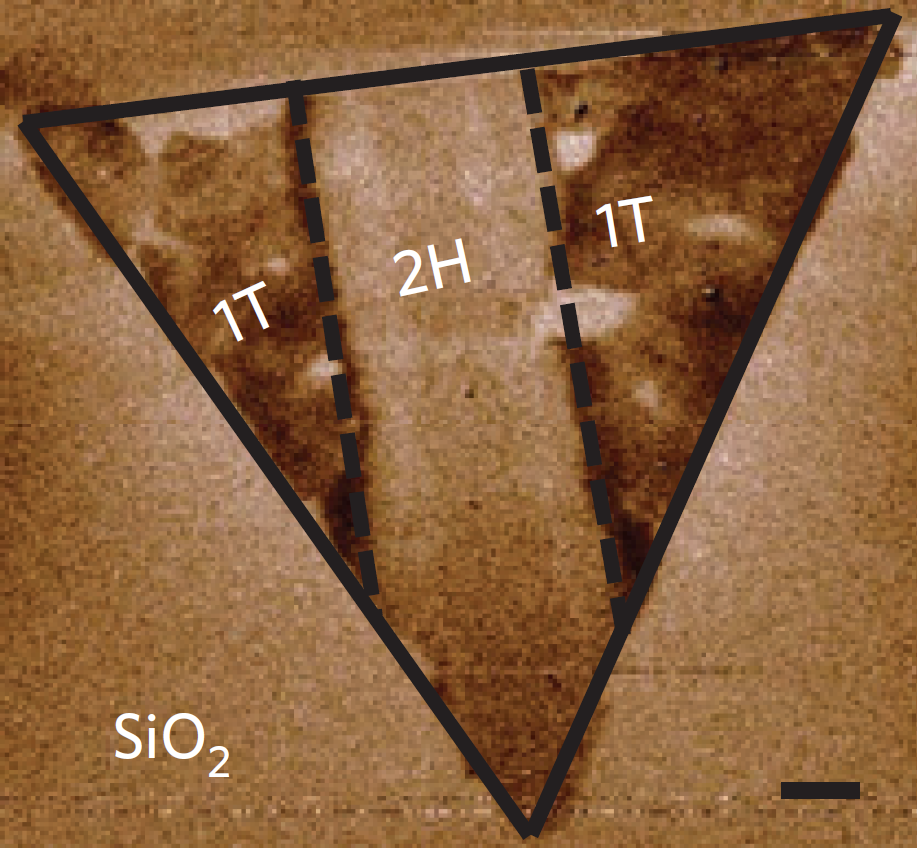
\includegraphics[scale=0.25]{1T'/Homojunction.png}
		\caption{Electrostatic force microscopy phase image of a monolayered MoS2 homojunction. Reproduced from \cite{Kappera2014}}
		\label{fig:1T'Homojunction}
	\end{center}
\end{figure}

\section{Conclusions}

In this chapter we have summarized the fundamental differences between 2H and 1T/1T’ phases of TMDCs with emphasis on the different crystalline phases and electronic properties along with different phenomena that can be enabled by the 1T’ phases. Additionally, we have laid out a short summary of the synthesis methods for the metastable 1T/1T’ phases.